\section{PyBullet}

PyBullet is a simulator built on the Bullet physics engine. Bullet's initial release dates back to 2006. Bullet engine was initially game, and graphics focused, but lately, with PyBullet, it has been increasingly popular among roboticists. We decided on using PyBullet for several strong reasons and overall satisfied by the performance and the features it offers. 

Firstly, PyBullet recently published their RL resources on Github \footnote{\url{https://bit.ly/3h1X7uU}}. These resources provide everything necessary to quickly start experimenting with any choice of robot, environment, and algorithm. Secondly, in RL robotics research, our reference papers are using PyBullet for their experiments \cite{Quillen2018} \cite{Breyer2018}. Therefore, it is more convenient to compare results using the same physical engine to avoid simulation differences. Thirdly, it has sizeable open-source support and free to use. 

On the other hand, based on Erez et al. performance tasks, which compares Bullet, Mujoco, ODE, and PhysX engines, Bullet is either at the last place or the one above the last position \ref{fig:BulletComp} figure. Similarly, they mention Bullet Engine's spring-damper system's incompatibility with the standard PD controller design \cite{Erez2015}.

Many open-source robotics learning resources migrating to PyBullet. This migration brings more open-source contributors who are more focused on Reinforcement Learning. For example, open-source contributors recently developed multi-threading GPU support to PyBullet. Also, Stable Baselines\footnote{\url{https://github.com/hill-a/stable-baselines}} creators implemented a RL training package under Bullet's Github repository\footnote{\url{https://bit.ly/3jqU7Kd}} \cite{stable-baselines}. 

In conclusion, PyBullet is the most actively developed physics engine among the three contenders. Thanks to the open-source community, any small bug is reported and solved quickly, missing in Gazebo and Mujoco. We assume more roboticists will migrate to PyBullet in the future. As a result of this, it will become a primary physics engine for robotics research. Despite research papers representing Pybullet engine performance as the worst among three, we have not noticed any significant failure in engine performance in practice.

\begin{figure}

    \begin{subfigure}{0.31\textwidth}
      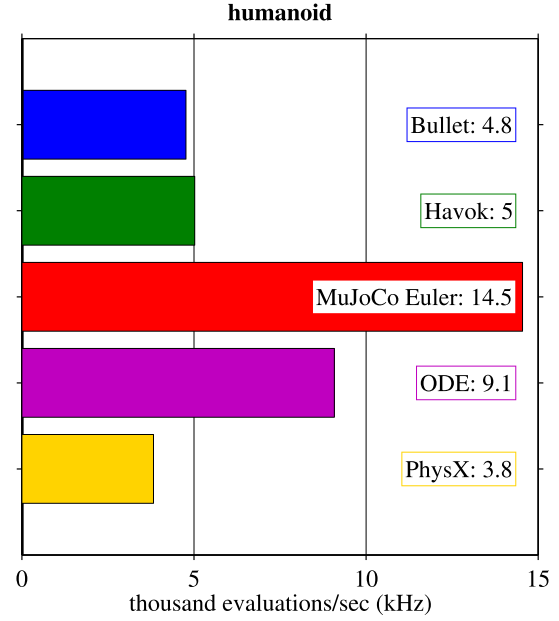
\includegraphics[width=\linewidth]{figures/BulletCom1.png}
      \caption{} \label{fig:1a}
    \end{subfigure}%
    \hspace*{\fill}   % maximize separation between the subfigures
    \begin{subfigure}{0.31\textwidth}
      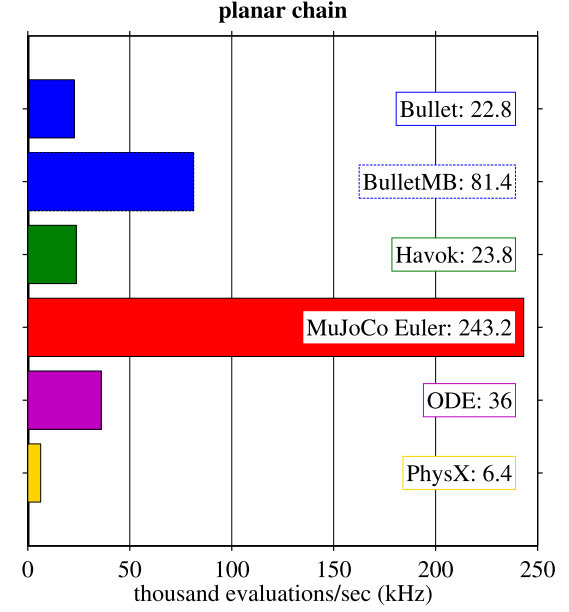
\includegraphics[width=\linewidth]{figures/BulletCom2.png}
      \caption{} \label{fig:1b}
    \end{subfigure}%
    \hspace*{\fill}   % maximize separation between the subfigures
    \begin{subfigure}{0.31\textwidth}
      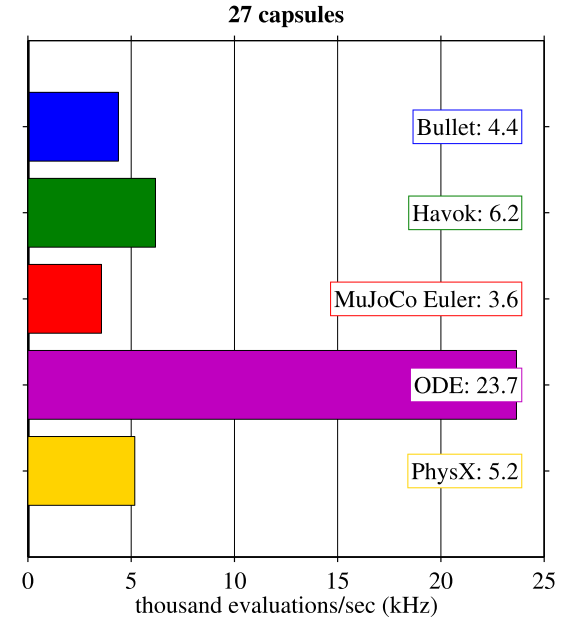
\includegraphics[width=\linewidth]{figures/BulletCom3.png}
      \caption{} \label{fig:1b}
    \end{subfigure}%

\caption{Comparing physics engine performances. Bullet is either at the last place or the one above the last position \cite{Erez2015} \label{fig:BulletComp}}
\end{figure}


\begin{figure}

    \begin{subfigure}{0.49\textwidth}
      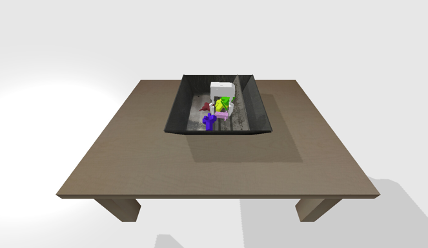
\includegraphics[width=\linewidth]{figures/PybulletEnv1.png}
      \caption{} \label{fig:1a}
    \end{subfigure}%
    \hspace*{\fill}   % maximize separation between the subfigures
    \begin{subfigure}{0.49\textwidth}
      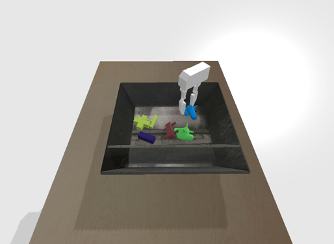
\includegraphics[width=\linewidth]{figures/PybulletEnv2.png}
      \caption{} \label{fig:1b}
    \end{subfigure}%

\caption{Screenshot from our trained hand model in Pybullet \label{fig:gripperbullet}}
\end{figure}
